%\documentclass[spanish]{beamer}
\documentclass{beamer}
\usepackage{pgf,pgfpages}
%\pgfpagesuselayout{4 on 1}[letterpaper,landscape,border shrink=0.5in]
\usepackage{algorithm,algorithmic}
%\usepackage{algorithm,algorithmicx}
%\usepackage[noend]{algpseudocode}
\usepackage{listings}
\lstset{basicstyle=\ttfamily,
	showstringspaces=false,
	commentstyle=\color{red},
	literate={á}{{\'a}}1
	{ã}{{\~a}}1
	{é}{{\'e}}1
	{É}{{\'E}}1
	{ó}{{\'o}}1
	{í}{{\'i}}1
	{ñ}{{\~n}}1
	{¡}{{!`}}1
	{¿}{{?`}}1
	{ú}{{\'u}}1
	{Í}{{\'I}}1
	{Ó}{{\'O}}1
}

\usepackage{beamerthemesplit}
\usepackage{color}
\usepackage[utf8]{inputenc}
\usepackage[spanish]{babel}
%\usepackage[latin1]{inputenc}
%\usepackage[pdftex]{graphicx}
%\usepackage{algorithm}
%\usepackage{algorithmic-C}
%\usepackage{algorithmic}
\usepackage{amsthm}
\usepackage{multicol}
\usepackage{multirow}
\usepackage{fancyvrb,relsize}
\usepackage{hhline}
\usepackage{tikz}
\usetikzlibrary{trees, shapes, calc}
\newcommand{\inputTikZ}[2]{%
	\scalebox{#1}{\input{#2}}
}

\usetheme{Warsaw} %Gueno
%\usetheme{Darmstadt} %OK!
% \usetheme{Frankfurt} %OK!
%\usetheme{Goettingen}
%\usetheme{Dresden}
%\usetheme{JuanLesPins} %OK!!
%\usetheme{Marburg}
%\usetheme{Montpellier}
%\usetheme{Rochester} %sobrio
%\usetheme{Singapore}
%\usetheme{Szeged}

%\usecolortheme{albatross}
%\usecolortheme{seahorse}
%\usecolortheme{beetle}
%\usecolortheme{crane}
%\usecolortheme{dolphin}
%\usecolortheme{dove}
%\usecolortheme{fly}
%\usecolortheme{lily} %Gueno
\usecolortheme{orchid}%Gueno
%\usecolortheme{rose}
%\usecolortheme{seagull}
%\usecolortheme{whale}


\DefineVerbatimEnvironment%
      {VerbatimNN}%
      {Verbatim}%
      {fontsize=\relsize{-1}}
\DefineVerbatimEnvironment%
      {VerbatimNNN}%
      {Verbatim}%
      {fontsize=\relsize{-2}}

\DefineVerbatimEnvironment%
      {VerbatimPseudo}%
      {Verbatim}%
      {numbers=left, fontsize=\relsize{-1}}
\DefineVerbatimEnvironment%
      {VerbatimPseudoReduced}%
      {Verbatim}%
      {numbers=left, fontsize=\relsize{-2}}
\DefineVerbatimEnvironment%
      {VerbatimPseudoReduced2}%
      {Verbatim}%
      {numbers=left, fontsize=\relsize{-3}}
\DefineVerbatimEnvironment%
      {VerbatimC}%
      {Verbatim}%
      {commandchars=@ªº, numbers=left, fontsize=\relsize{-1}}
\DefineVerbatimEnvironment%
      {VerbatimReducedC}%
      {Verbatim}%
      {commandchars=@ªº, numbers=left, fontsize=\relsize{-2}}
\DefineVerbatimEnvironment%
      {VerbatimReduced2C}%
      {Verbatim}%
      {commandchars=@ªº, numbers=left, fontsize=\relsize{-3}}



%\AtBeginSubsection[]
%{
% \begin{frame}
% \frametitle{Sinopsis}
% Aqui decides: cada seccion y subseccion:
% \tableofcontents[currentsection,currentsubsection]
 %O solamente la seccion (Solo uno de ellos)
%\tableofcontents[currentsection]
% \end{frame}
%}

% Si quieres que todo por default aparezca de poco en poco
% descomenta esta linea
%\beamerdefaultoverlayspecification{<+->}

\setbeamertemplate{footline}{\hfill\insertframenumber/\inserttotalframenumber}
\setbeamertemplate{navigation symbols}{}

\setbeamercovered{transparent}

\title{ELO320 - Estructuras de Datos y Algoritmos\\Tipos de Datos Abstractos\\Tablas Hash}
%\subtitle{Ingeniería Civil Telemática UTFSM}
\author{Dr. Nicolás Gálvez R.\\{\small nicolas.galvez@usm.cl}}
\institute{Ing. Civil Telemática - Departamento de Electrónica}
\titlegraphic{
\includegraphics[scale=.18]{images/logoutfsm}}
\date{1er Semestre 2022}

\begin{document}

\frame{\titlepage}

%\section*{Sinopsis}
%\frame{  \frametitle{Sinopsis}\tableofcontents[pausesections]}
%
%

\section{Árbol binario de búsqueda}



\begin{frame}[fragile]
 \frametitle{Tablas Hash}
\small
Las tablas hash son una estructura de datos en la que las operaciones de inserción, búsqueda y eliminación son muy rápidas, independientemente del
tamaño de los datos.
\begin{itemize}
\item Arreglo Asociativo.
\item Pares llave-valor.
\item Llaves únicas.
\item Función hash.
\end{itemize}

\begin{center}
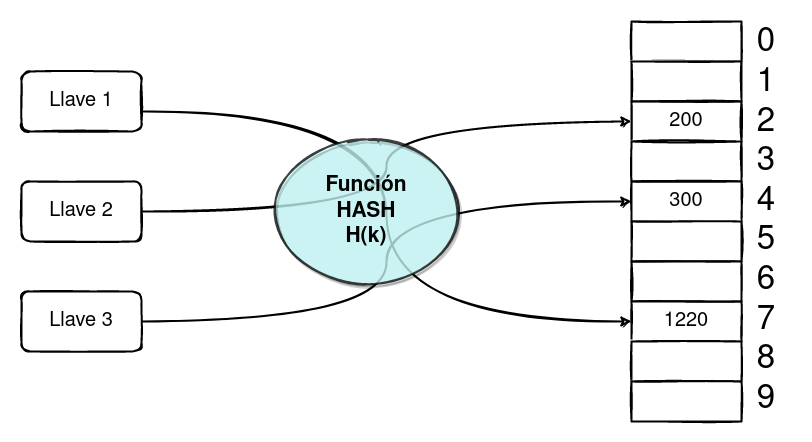
\includegraphics[width=.7\linewidth]{images/hash1}
\end{center}

\end{frame}

\begin{frame}[fragile]
 \frametitle{Tablas Hash}
\small
Diseñadas originalmente para resovler el \textbf{problema de búsqueda}, las Tablas Hash es una estructura basada en arreglos, pero sin trabajar directamente con el índice de ellos.  Algunos usos:
\begin{itemize}
\item Diccionarios en Python.
\item Map en C++.
\item Sistemas de contraseñas (encriptación).
\item Memoria Caché. 
\end{itemize}

\begin{center}
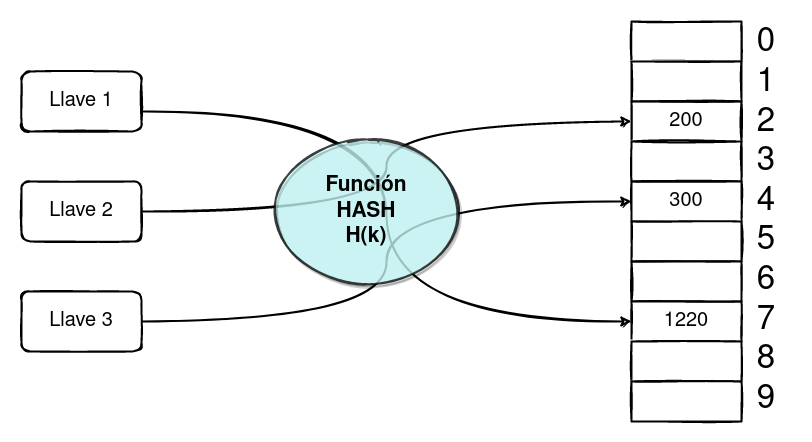
\includegraphics[width=.65\linewidth]{images/hash1}
\end{center}

En \textbf{promedio}, la complejidad de los métodos de Tablas Hash es \textbf{$\mathcal{O}(1)$}. Lo veremos en la próxima clase.

\end{frame}

\begin{frame}[fragile]
 \frametitle{Tablas Hash}
\small
Las tablas hash se componen de un conjunto de datos $D$ formado por tuplas de información llave-valor $(k.v)$, y un arreglo $A$ en donde se almacenan los valores.
$$ D = \{(k_1,v_1), (k_2,v_2), \dots (k_n, v_n) \} $$

El índice del arreglo asociado a un par se obtiene aplicando una función de transformación $H(k)$, llamada \textbf{función hash}. 
$$ H: D_k \rightarrow \{1, 2, 3, \dots, m\}$$
$$ A[H(k_i)] = v_i;\ \forall i \in \{1,2,3,\dots,n\} $$

\begin{center}
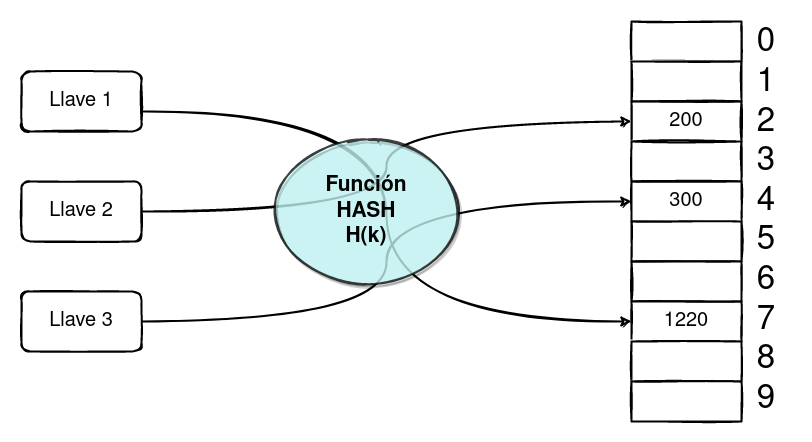
\includegraphics[width=.65\linewidth]{images/hash1}
\end{center}
\end{frame}

\begin{frame}[fragile]
 \frametitle{Tabla Hash: Métodos}

\begin{exampleblock}{Métodos}
\begin{lstlisting}[language=C, basicstyle=\tiny, escapeinside={|}{|}]
int search(int array[10], char *key){
	return array[hash(key)];
}

void insert(int array[10], char *key, int value){
	array[hash(key)] = value;	
}

void remove(int array[10], char *key){
	array[hash(key)] = NULL;
}

\end{lstlisting}
\end{exampleblock}
\end{frame}

\section{Conflictos}
\begin{frame}[fragile]
 \frametitle{Tablas Hash: Conflicto}
\small
Las tablas hash, al trabajar con un arreglo fijo, poseen un gran problema. Dos llaves pueden ser asignadas a un mismo indice por la tabla hash.
Esto es lo que se llama \textbf{conflicto}.

\begin{center}
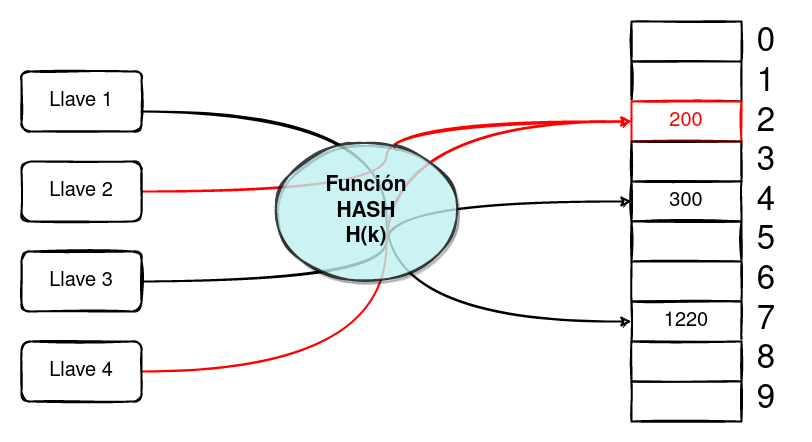
\includegraphics[width=.75\linewidth]{images/hashconflicto}
\end{center}

Existen variadas técnicas para su resolución, que veremos a continuación.

\end{frame}

\section{Conflictos}
\begin{frame}[fragile]
 \frametitle{Tablas Hash: Hashing Abierto}
\small
Una de las formas de resolver los conflictos es el Hashing Abierto. El arreglo fijo, pasa a ser un arreglo de punteros, los cuales establecen una lista para almacenar los nodos en conflicto.

\begin{center}
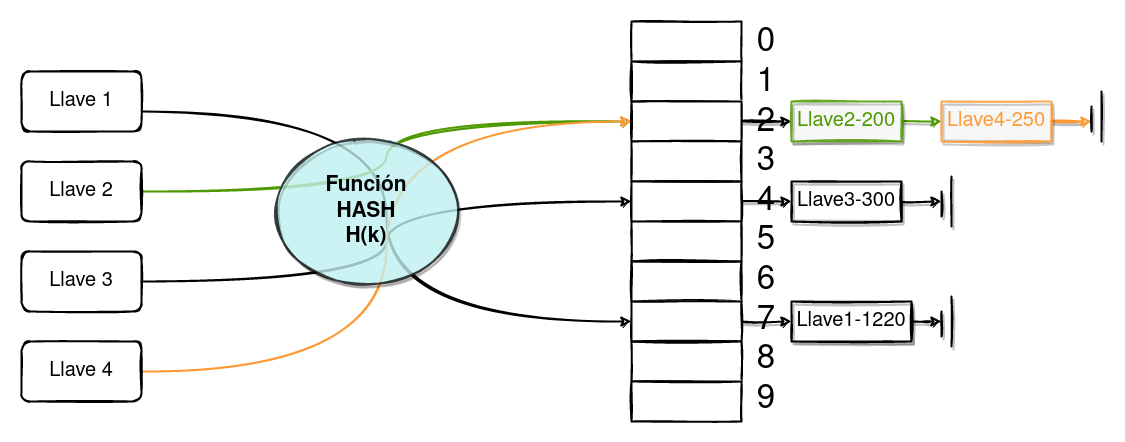
\includegraphics[width=.9\linewidth]{images/hashabierto}
\end{center}

La búsqueda entonces es doble, en el arreglo y en la lista. Para evitar confusiones, en los nodos de las lista se guarda el par (llave, valor).

\end{frame}

\begin{frame}[fragile]
 \frametitle{Tablas Hash: Hashing Cerrado}
\small
Otra for de resolución es el Hashing Cerrado. En donde existen corrimientos de la posición de inserción si hay un conflicto. Esto evita el uso de estructuras de datos adiciones, pero habrá que tener cuidados son los overflow de memoria.

\begin{center}
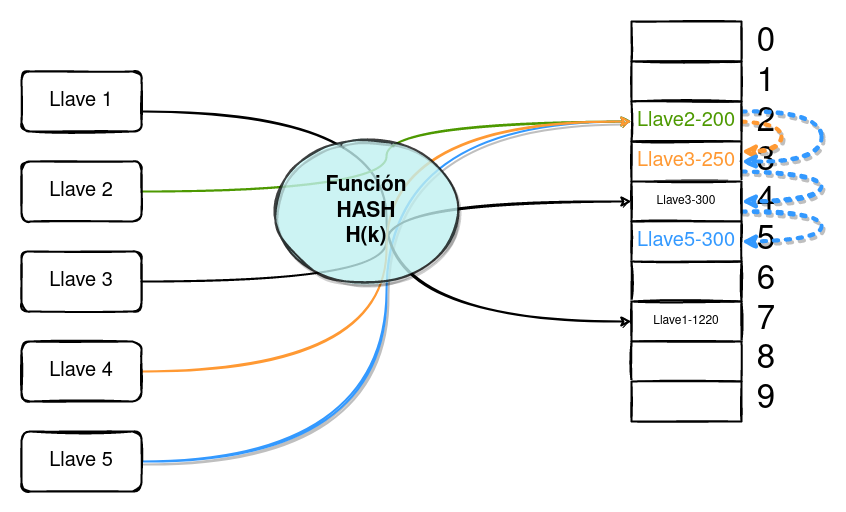
\includegraphics[width=.9\linewidth]{images/hashcerrado1}
\end{center}
\end{frame}

\begin{frame}[fragile]
 \frametitle{Tablas Hash: Hashing Cerrado}
\small
La primera técnica de Hashing Cerrado, busca insertar el dato en el casillero disponible más cercano.

\begin{center}
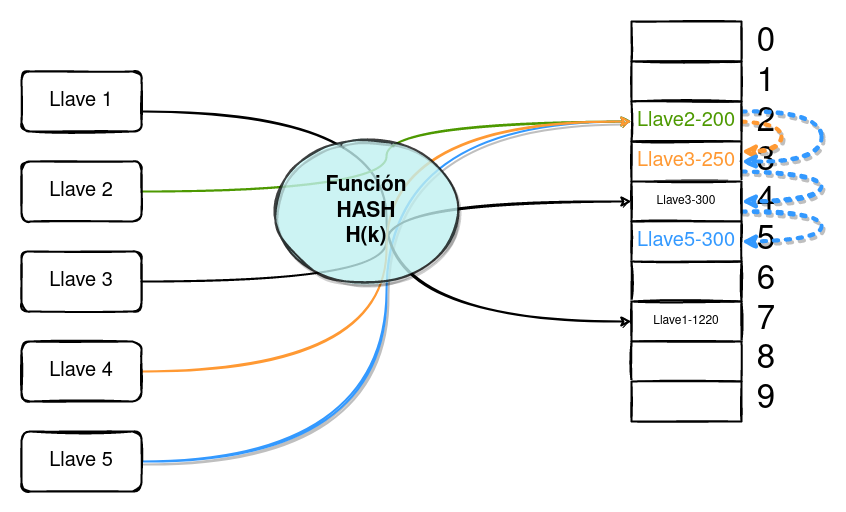
\includegraphics[width=.8\linewidth]{images/hashcerrado1}
\end{center}

La búsqueda, por lo tanto, sigue un proceso similar: parte de la posición entregada por la función hash, avanzando hasta encontrar el dato correcto.

\end{frame}

\begin{frame}[fragile]
 \frametitle{Tablas Hash: Hashing Cerrado}
\small
Un problema de lo anterior es que los datos tienen a agruparse alrederor de las inserciones limpias. Para evitar esto, la misma técnica se aplica pero buscando cada $C$ casilleros. 

\begin{center}
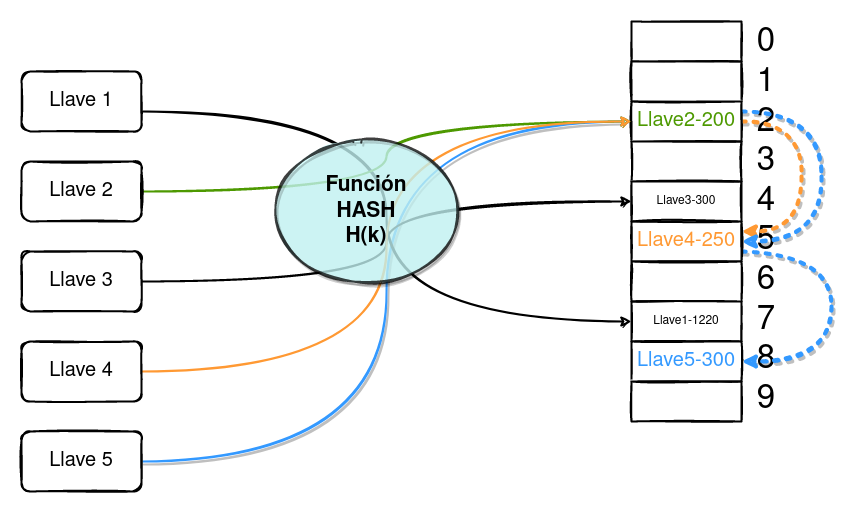
\includegraphics[width=.8\linewidth]{images/hashcerrado2}
\end{center}

La búsqueda, por lo tanto, sigue un proceso similar: parte de la posición entregada por la función hash, avanzando en $C$ casilleros hasta encontrar el dato correcto.

\end{frame}

\section{Funciones Hash}
\begin{frame}[fragile]
 \frametitle{Tablas Hash: Funciones Hash}
\small Uno de los grandes desafíos en la implementación de tablas hash, es la creación de una función idonea para la transformación llave a índice del arreglo.

Se busca que sea:
\begin{itemize}
\item Simple $\rightarrow$ facil implementación.
\item Uniforme $\rightarrow$ que las claves tengan la misma chance de ser mapeado a cualquier índice.
\end{itemize}

Técnicas heurísticas:
\begin{itemize}
\item Método de la División.
\item Método de la Multiplicación.
\end{itemize}

\end{frame}

\begin{frame}[fragile]
 \frametitle{Tablas Hash: Método de la División}
\small
En este método las claves son transformadas en índices del arreglo mediante el uso de resto aritmético o módulo sobre

$$ h(k) = k\ \mathrm{mod}\ m$$

La recomendación general, es usar un largo de arreglo $m$ que no esté relacionado con la distribución de llaves. Por lo general, un número primo. 
\end{frame}

\begin{frame}[fragile]
 \frametitle{Tablas Hash: Método de la Multiplicación}
\small
Este método se compone de los siguientes pasos:
\begin{enumerate}
\item Multiplicar la llave por una constante $\alpha \in ]0,1[$.
\item Obtener la parte fraccional del resultado de la multiplicación.
\item Multiplicar dicha parte por el tamaño del arreglo $m$
\item Truncar el resultado final.
\end{enumerate}

$$ h(k) = \lfloor m \times  ((k\times \alpha)\ \mathrm{mod}\ 1) \rfloor $$ 

En este caso el tamaño de m, no es crítico. Esto permite que comunmente se use una potencia de dos para el tamaño del arreglo: $m = 2^p$.
\end{frame}

\begin{frame}[fragile]
 \frametitle{Tablas Hash: Uso de Strings}
\small
En general las funciones de hash trabajan con valores numéricos enteros. ¿Cómo se puede trabajar con strings? Utilizamos los valores ASCII de los caracteres para generar un valor numérico.

\begin{exampleblock}{String = "hash"}
\footnotesize
\begin{itemize}
\item Valores ASCII:
$$h = 104,\ a=97,\ s=115$$
\item Suma de valores: 
$$104+97+115+104 = 420 $$
\item Radix-128:
$$(104\times 128^3) + (97 \times 128^2) + (115\times 128^1) + (104\times 128^0) = 219707880 $$
\end{itemize}

\end{exampleblock}

\end{frame}


%\begin{frame}[fragile]
% \frametitle{ABB: Árbol binario de búsqueda}
%\small
%Por ejemplo, es fácil determinar el lugar y posición de los valores en un intervalo. 
%
%\begin{center}
%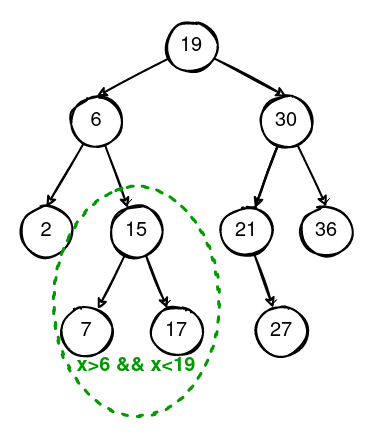
\includegraphics[width=.35\linewidth]{images/abb3}
%\end{center}
%
%\begin{itemize}
%\item \textbf{¿Cómo determinan el sucesor y predecesor de un padre?}\\
%{\color{red}{Sucesor: buscar en la derecha, todo hacia la izquierda.}}\\
%{\color{blue}{Antecesor: buscar en la izquierda, todo hacia la derecha.}} \\
%\item \textbf{¿Cuál es su principal característica?}\\
%{\color{red}{Siempre tendrán a lo más un hijo.}}
%\end{itemize}
%\end{frame}
%
%
%\begin{frame}[fragile]
% \frametitle{ABB: Operaciones}
%\small Las operaciones más comunes de los ABB son:
%
%\begin{itemize}
%\item \texttt{init()}: Inicializar el árbol (root == NULL).
%\item \texttt{size()}: Cantidad de elementos en el árbol.
%\item \texttt{x\_preorden()}: Operación x en pre-orden.
%\item \texttt{x\_inorden()}: Operación x en in-orden. 
%\item \texttt{x\_postorden()}: Operación x en post-orden. 
%\item \texttt{search()}: Buscar un elemento en el árbol.
%\item \texttt{insert()}: Insertar un elemento en el árbol.
%\item \texttt{delete()}: Eliminar un elemento en el árbol.
%\item \texttt{clear()}: Limpiar el árbol.
%\end{itemize}
%\end{frame}
%
%\begin{frame}[fragile]
% \frametitle{ABB: Recorrer}
%\small
%¿Como se imprimirían los datos del siguiente árbol con recorrido pre-orden, in-orden y post-orden?
%
%\begin{center}
%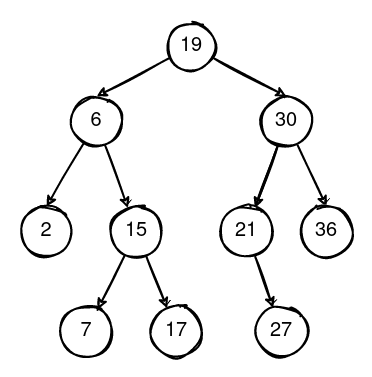
\includegraphics[width=.45\linewidth]{images/abb1}
%\end{center}
%
%\pause
%\begin{itemize}
%\item Pre-orden: 19 - 6 - 2 - 15 - 7 - 17 - 30 - 21 - 27 - 36 \pause
%\item In-orden: 2 - 6 - 7 - 15 - 17 - 19 - 21 - 27 - 30 - 36 \pause
%\item Post-orden: 2 - 7 - 17 - 15 - 6 - 27 - 21 - 36 - 30 - 19 
%\end{itemize}
%
%
%\end{frame}
%
%
%\begin{frame}[fragile]
% \frametitle{ABB: Buscar}
%Comenzaremos con la función básica \texttt{search()}: Buscar un elemento en el árbol.
%
%\begin{center}
%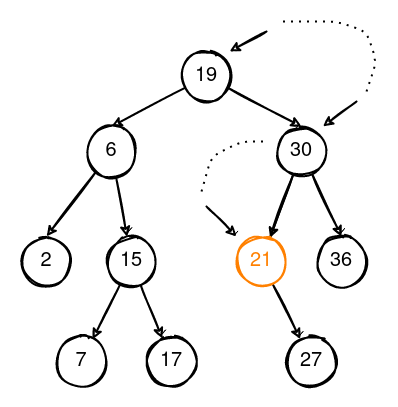
\includegraphics[width=.35\linewidth]{images/abb-search}
%\end{center}
%
%Se puede hacer de dos formas:
%\begin{itemize}
%\item Usando un puntero para recorrer el árbol.
%\item \textbf{Recursivamente}.
%\end{itemize}
%\end{frame}
%
%\begin{frame}[fragile]
% \frametitle{ABB: Buscar}
%
%\begin{exampleblock}{Recursivamente}
%\begin{lstlisting}[language=C, basicstyle=\tiny, escapeinside={|}{|}]
%int * search(nodo_t * raiz, int value){ 
%
%	if(raiz == NULL || raiz->dato == value) //{} omitidas
%		return raiz;
%	else if(value < raiz->dato)
%		return search(raiz->hijo_izq, value);
%	else if(value > raiz->dato) // else
%		return search(raiz->hijo_der, value);
%	
%}
%\end{lstlisting}
%\end{exampleblock}
%
%\begin{block}{Usando Puntero}
%\begin{lstlisting}[language=C, basicstyle=\tiny, escapeinside={|}{|}]
%int * search(nodo_t * raiz, int value){
%	
%	nodo_t * rec = raiz;
%	while(rec!=NULL){
%		if(rec->dato == value){
%			return rec;
%		}else if(value < rec->dato){
%			rec = rec->hijo_izq;
%		}else if(value > rec->dato){
%			rec = rec->hijo_der;
%		}
%	return rec; // NULL si no lo encuentra o arbol vacío
%}
%\end{lstlisting}
%\end{block}%
%\end{frame}
%
%\begin{frame}[fragile]
% \frametitle{ABB: Insertar}
%\small
%Para poder insertar debemos buscar primero el lugar donde debe realizarse la inserción. La idea es \textbf{mantener} el orden de nuestro ABB.
%
%\begin{center}
%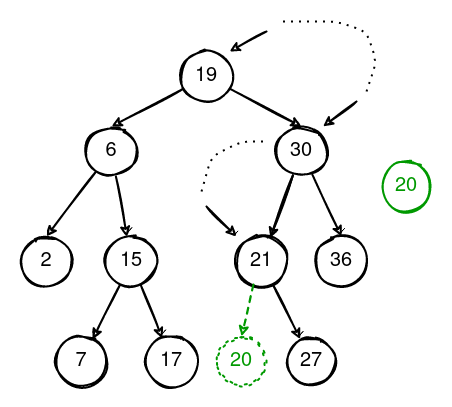
\includegraphics[width=.45\linewidth]{images/abb-insert}
%\end{center}
%
%Nota: Si nuestro árbol no acepta elementos repetidos, al encontrar el valor se detiene.
%
%\end{frame}
%
%\begin{frame}[fragile]
% \frametitle{ABB: Insertar}
%\begin{exampleblock}{Recursivamente}
%\begin{lstlisting}[language=C, basicstyle=\tiny, escapeinside={|}{|}]
%void insert(nodo_t ** raiz, int value){ 
%
%	if(*raiz == NULL){
%		*raiz = malloc(sizeof(node_t));
%		(*raiz)-> dato = value;
%		(*raiz)->hijo_izq = NULL;
%		(*raiz)->hijo_der = NULL;
%
%	}else if(value < (*raiz)->dato){
%		insert(&((*raiz)->hijo_izq), value);
%
%	}else if(value > (*raiz)->dato){
%		insert(&((*raiz)->hijo_der), value);
%	}
%}
%\end{lstlisting}
%\end{exampleblock}
%\end{frame}
%
%\begin{frame}[fragile]
% \frametitle{ABB: Insertar}
%Cree el árbol binario que represente la siguiente secuencia de enteros: 
%$$ 10 - 5 - 7 - 14 - 12 - 18 - 15 $$\pause
%\begin{alertblock}{Spoiler}
%\begin{center}
%\visible<.(1)>{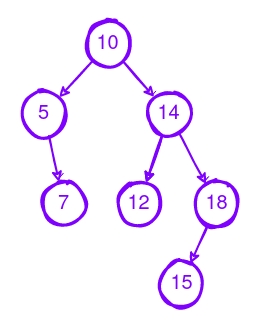
\includegraphics[width=.35\linewidth]{images/abb-insert-example}}
%\end{center}
%\end{alertblock}
%\end{frame}
%
%\begin{frame}[fragile]
% \frametitle{ABB: Eliminar}
%\small
%Al igual que en insertar, deberemos buscar el nodo a eliminar. Pero para poder eliminarlo, tendremos que considerar los siguientes casos:
%
%\begin{itemize}
%\item Nodo objetivo es una hoja (no tiene hijos).
%\item Nodo objetivo tiene un sólo hijo.
%\item Nodo objetivo tiene dos hijos.
%\end{itemize}
%
%\end{frame}
%
%\begin{frame}[fragile]
% \frametitle{ABB: Eliminar hoja.}
%\small
%Es el caso más sencillo, solo corresponde a liberar el nodo desde el puntero del padre.
%
%\begin{center}
%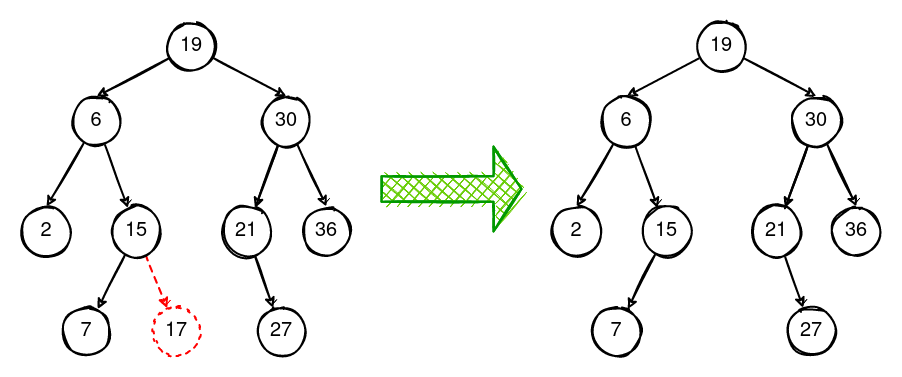
\includegraphics[width=.9\linewidth]{images/abb-delete-nochild}
%\end{center}
%\end{frame}
%
%\begin{frame}[fragile]
% \frametitle{ABB: Eliminar nodo con 1 hijo.}
%\small
%Caso intermedio. acá se elimina el nodo encontrado, pero su posición es ocupada por su único hijo. Se eleva ese sub-árbol, un nivel.
%
%\begin{center}
%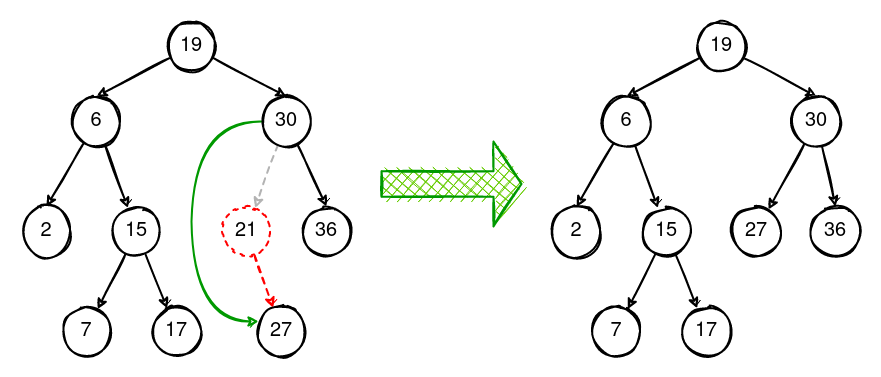
\includegraphics[width=.9\linewidth]{images/abb-delete-onechild}
%\end{center}
%\end{frame}
%
%\begin{frame}[fragile]
% \frametitle{ABB: Eliminar nodo con 2 hijos.}
%\small
%Caso recursivo o iterativo. Cuenta de dos pasos:
%\begin{itemize}
%\item Reemplazar el nodo objetivo por una copia de su sucesor o antecesor (uds. eligen).
%\item Borrar el sucesor o antecesor original.
%\end{itemize}
%
%\begin{center}
%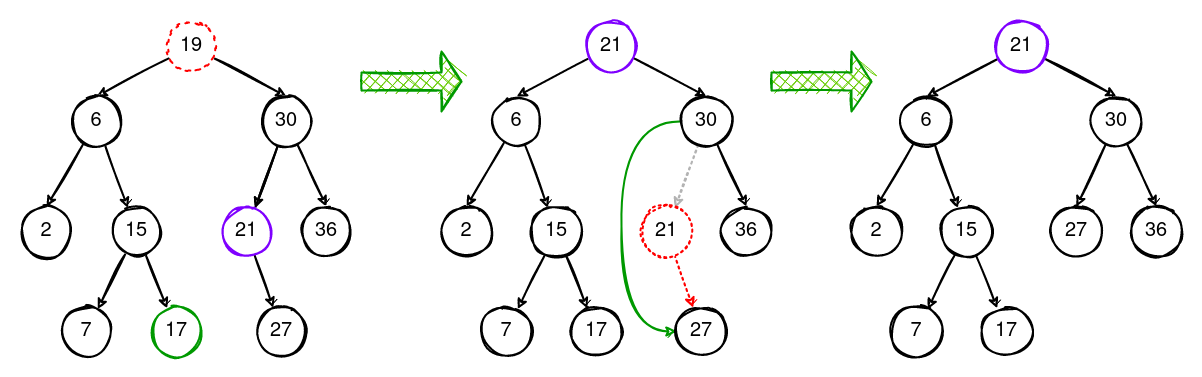
\includegraphics[width=\linewidth]{images/abb-delete-twochild}
%\end{center}
%\end{frame}
%
%
%
%\begin{frame}[fragile]
% \frametitle{ABB: Insertar}
%\begin{exampleblock}{Recursivamente}
%\begin{lstlisting}[language=C, basicstyle=\tiny, escapeinside={|}{|}]
%int delete(nodo_t ** raiz, int value){ 
%	// ¿Cómo lo programan?
%	// Necesitarán alguna función extra.
%}
%\end{lstlisting}
%\end{exampleblock}
%\end{frame}
%
%\begin{frame}[fragile]
% \frametitle{Ejercicios}
%\begin{itemize}
%\item Para el siguiente conjunto $\{1, 4, 5, 10, 16, 17, 21\}$, dibuje árboles binarios de búsqueda con altura 2, 3, 4, 5, y 6.
%\item Escriba funciones recursivas para recorrer un árbol binario de búsqueda en pre-orden y post-orden.
%\item Asuma que tiene números entre 1 y 1000 en un árbol binario de búsqueda y quiere buscar el nodo 363. ¿Cuál de las siguientes secuencias de nodos NO podría ser una secuencia de nodos examinados en el árbol para llegar al nodo 363?
%\begin{enumerate}
%\item 2, 252, 401, 398, 330, 344, 397, 363.
%\item 924, 220, 911, 244, 898, 258, 362, 363.
%\item 925, 202, 911, 240, 912, 245, 363.
%\item 2, 399, 387, 219, 266, 382, 381, 278, 363.
%\item 935, 278, 347, 621, 299, 392, 358, 363.
%\end{enumerate}
%\end{itemize}
%\end{frame}

\end{document}
